\chapter{Coverage}\label{chap:coverage}

\section{ Strategy }
The coverage method used is boustrophedon, meaning “the way of the ox” from the
plowing pattern of old days. The advantage of this strategy is that it ensures
full coverage of a room with no obstacles and it is simple.

It is clear that when actually implemented on a robot, it must be supported by
online sensors to cope with the obstacles present in the room, but for the
purpose of estimating the distance travelled by such a robot, it gives a best
case route.

\begin{figure}[htb]
	\centering
	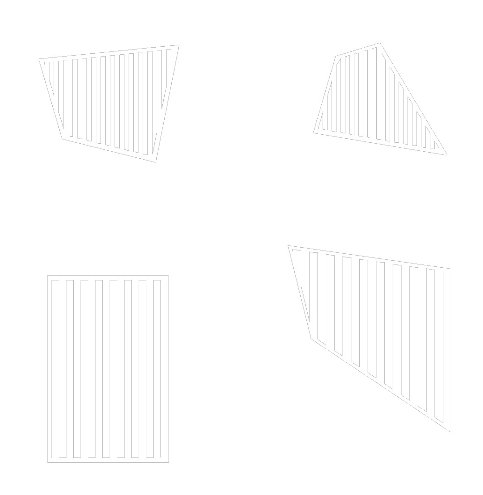
\includegraphics[width=0.3\paperwidth,trim=0 0 0
	0]{graphics/covered_cells.jpg}
	%trim=l b r t (can cut off from every side)
	\caption{Shows example cells covered}
	\label{fig:covered_cells}			
\end{figure}

\subsection{Algorithm}
The algorithm developed for covering follows the points listed in
\ref{fig:boustrophedon}. The algorithm assumes the cell has been shrunk so the
area given in the cell structure represents the free spae in which the robots center
can move.

The algorithm first constructs a polygon from the cell data. Then the cell is
swept by discrete vertical lines for every distance given by radius. This way a
list is constructed holding the points where the sweeplines intersect the cell
polygon, thus giving the robots turning points. Finally the list is sorted to
reflect the order in which the turning points should be visited.

\begin{algorithm}
\caption{Boustrophedon coverage}\label{fig:boustrophedon}
\begin{algorithmic}[0]
\State \textbf{Input:}
\State cell\Comment{Structure holding vertices and edges}
\State radius\Comment{The radius covered by the robot}
\State list\Comment{empty list for returning the route}
\State \textbf{Output:}
\State distance\Comment{the lapsed distance}
\end{algorithmic}
\begin{algorithmic}[1]
\Function{cover area}{$cell$ , $radius$ , $points$}
\For {each edge in cell}
\State push line segment to $polygon$\Comment{This constructs a polygon shaped
as the cell}
\EndFor
\While{$sweepline$ inside $polygon$}
\State construct next $sweepline$
\State find intersections with $polygon$
\State push intersections to $points$
\EndWhile
\For {each point in $points$}
\State order $points$\Comment{up,down,up,down sequence}
\EndFor
\For {each point in $points$}
\State remove dublicates\Comment{in case intersection is a vertice}
\EndFor
\For {each point in $points$}
\State calculate $distance$
\EndFor
\State \textbf{return} $distance$
\EndFunction
\end{algorithmic}
\end{algorithm}

\subsection{ Running time }
The running time of this algoritm depends on the number of turningpoints in the
returned path and theese again depends on the width of the cell and the radius
of the robot.

\begin{equation}
n = 2 \cdot \frac{width}{radius}
\end{equation}

Finding the point requires finding the possible intersections between a
sweepline and the cell polygon. Since most cells are polygons of four vertices
this means on average checking each sweepline against four lines or two checks
per turning point. Checking the intersection between two lines means solving the
equaled line equasions and is thus done in constant time giving this problem a
complexity of O(n).

Ordering the list means iterating the list and reordering the points not
fulfilling the criteria. Since swapping two entries of a vector is done in
constant time, the operation is done in linear time.

Checking for dublicates means iterating the list and for each point checking the
rest of the list for similar points. This operation is done i quadratic time.

Calculating the travelled distance is done by iterating through the list and
adding up all the distances. Finding the distance between two points is done in
constant time and thus the complexity of this problem is O(n).

\subsection{Conclusion}
Overall analysis of the algorithm thus shows that it runs in quadratic time due
to the dublicate check and thus any effort to optimize the algorithm should
start here, but since most cells are relatively small, the problem is also
small.
